\bookchapter{0}{Why control?}{How this book began — with a helicopter on Mars — and what control theory is, where it came from and why a drone is the place to learn it.}
\label{ch:intro}

\lead{This book began on Mars. On 19~April 2021 a helicopter not much bigger than a toy lifted itself off the ground of another planet, hovered for half a minute and landed again. I watched it happen, and it fascinated me completely. This chapter tells that story first. Then it says what control theory is — the science that made the flight possible, and the subject of this book.}

\section{A helicopter on Mars}\index{Ingenuity (Mars helicopter)}

I followed the flights of Ingenuity, NASA's helicopter on Mars, as the news of each one arrived, and I was completely taken by them. It is hard to say how strongly a piece of engineering can move a person, but this one moved me. A machine of less than two kilograms, made by people, flying by itself through the thin air of a world where no person has ever stood — and doing it not once, as planned, but again and again. What I felt most was admiration: for the people who built it, and above all for the quiet power of the thing that kept it in the air, its control system. That admiration is the reason this book exists.

\sidecapfig{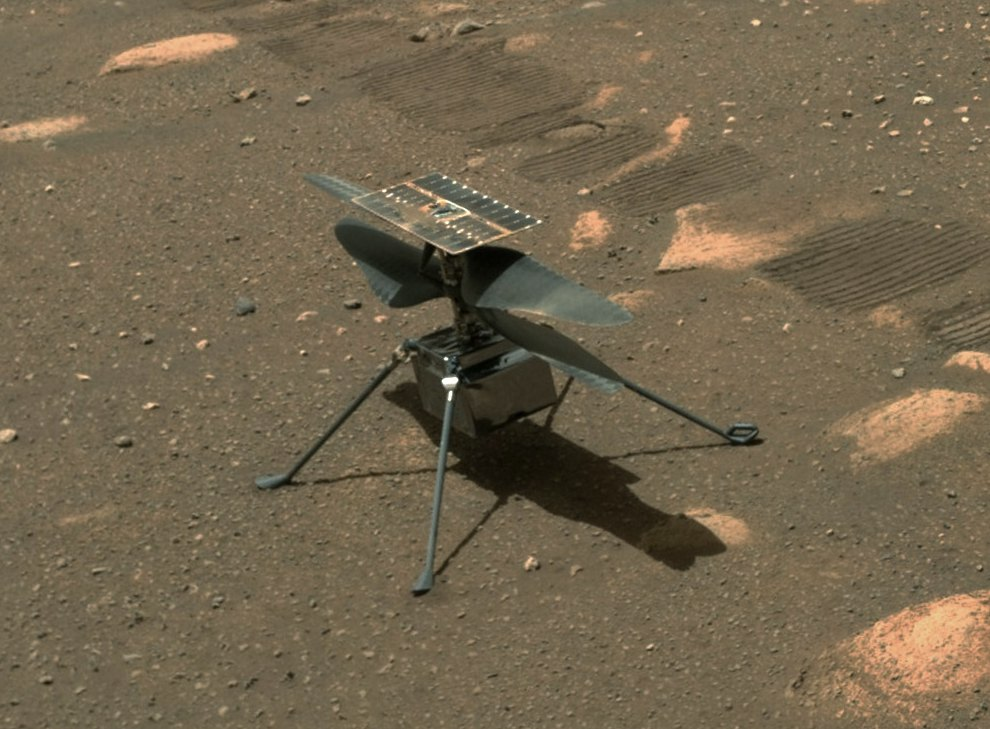
\includegraphics[width=\linewidth]{photos/ingenuity-mars}}
  {Ingenuity on the floor of Jezero crater, April 2021, photographed by the Perseverance rover. The two rotors, \SI{1.2}{m} across, turn in opposite directions; the solar panel on top charges its batteries. \hyperref[credit:ingenuity-mars]{\textsc{credit}}}
  {fig:intro-ingenuity}

Ingenuity reached Mars on 18~February 2021, folded under the belly of the Perseverance rover, which landed in Jezero crater. In early April the rover set it down on the ground (Figure~\ref{fig:intro-ingenuity}) and drove away, and the helicopter had to survive its first freezing night alone, on the power of its own small solar panel.

The engineering problem was extreme. The atmosphere of Mars has less than one per cent of the density of the air on Earth: a rotor there pushes against almost nothing. Ingenuity's answer was a pair of rotors \SI{1.2}{m} across, turning in opposite directions at about 2400 revolutions per minute, above a body of \SI{1.8}{kg}. And nobody could fly it. A radio signal needs several minutes to travel between Earth and Mars, up to about twenty-two, so there could be no pilot with a joystick, not even a patient one. Ingenuity had to fly itself. A camera looking down at the ground and inertial sensors told it where it was and how it was moving, and a computer built around a processor designed for smartphones closed the loop, many times every second, from sensors to rotors and back.

The first flight came on 19~April 2021. The helicopter rose about three metres, hovered and came down again, some thirty-nine seconds in all: the first powered, controlled flight of an aircraft on another planet. The patch of ground it flew from was named Wright Brothers Field, and the helicopter carried a small piece of the fabric that had covered the wings of the Wright brothers' Flyer in 1903.\marginphoto{ingenuity-wright}{The swatch of Wright Flyer fabric that flew on Ingenuity, photographed at JPL before launch.} Its own navigation camera took the first picture of Figure~\ref{fig:intro-shadows}: its shadow on the ground of Mars.

Ingenuity was meant to make at most five flights in thirty days, to show that flight on Mars was possible at all. It made seventy-two, over almost three years. It flew for 128.8~minutes in total, covered \SI{17}{km}, climbed as high as \SI{24}{m}, reached \SI{10}{m/s}, and became a scout for the rover, looking ahead at the ground it would have to cross.

\begin{figure}[tbp]
  \noindent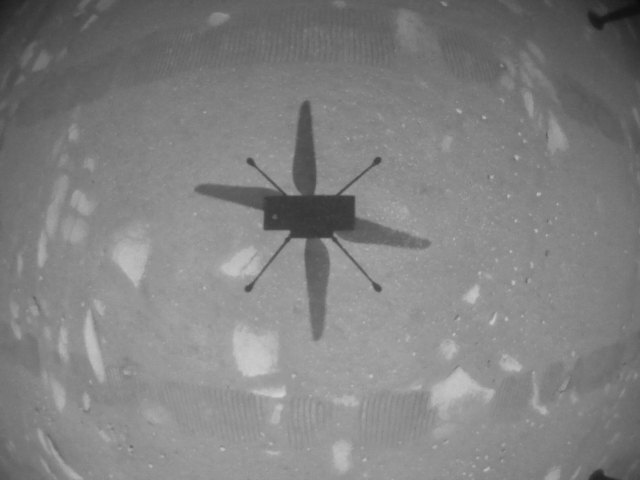
\includegraphics[height=40mm]{photos/ingenuity-shadow}\hfill
  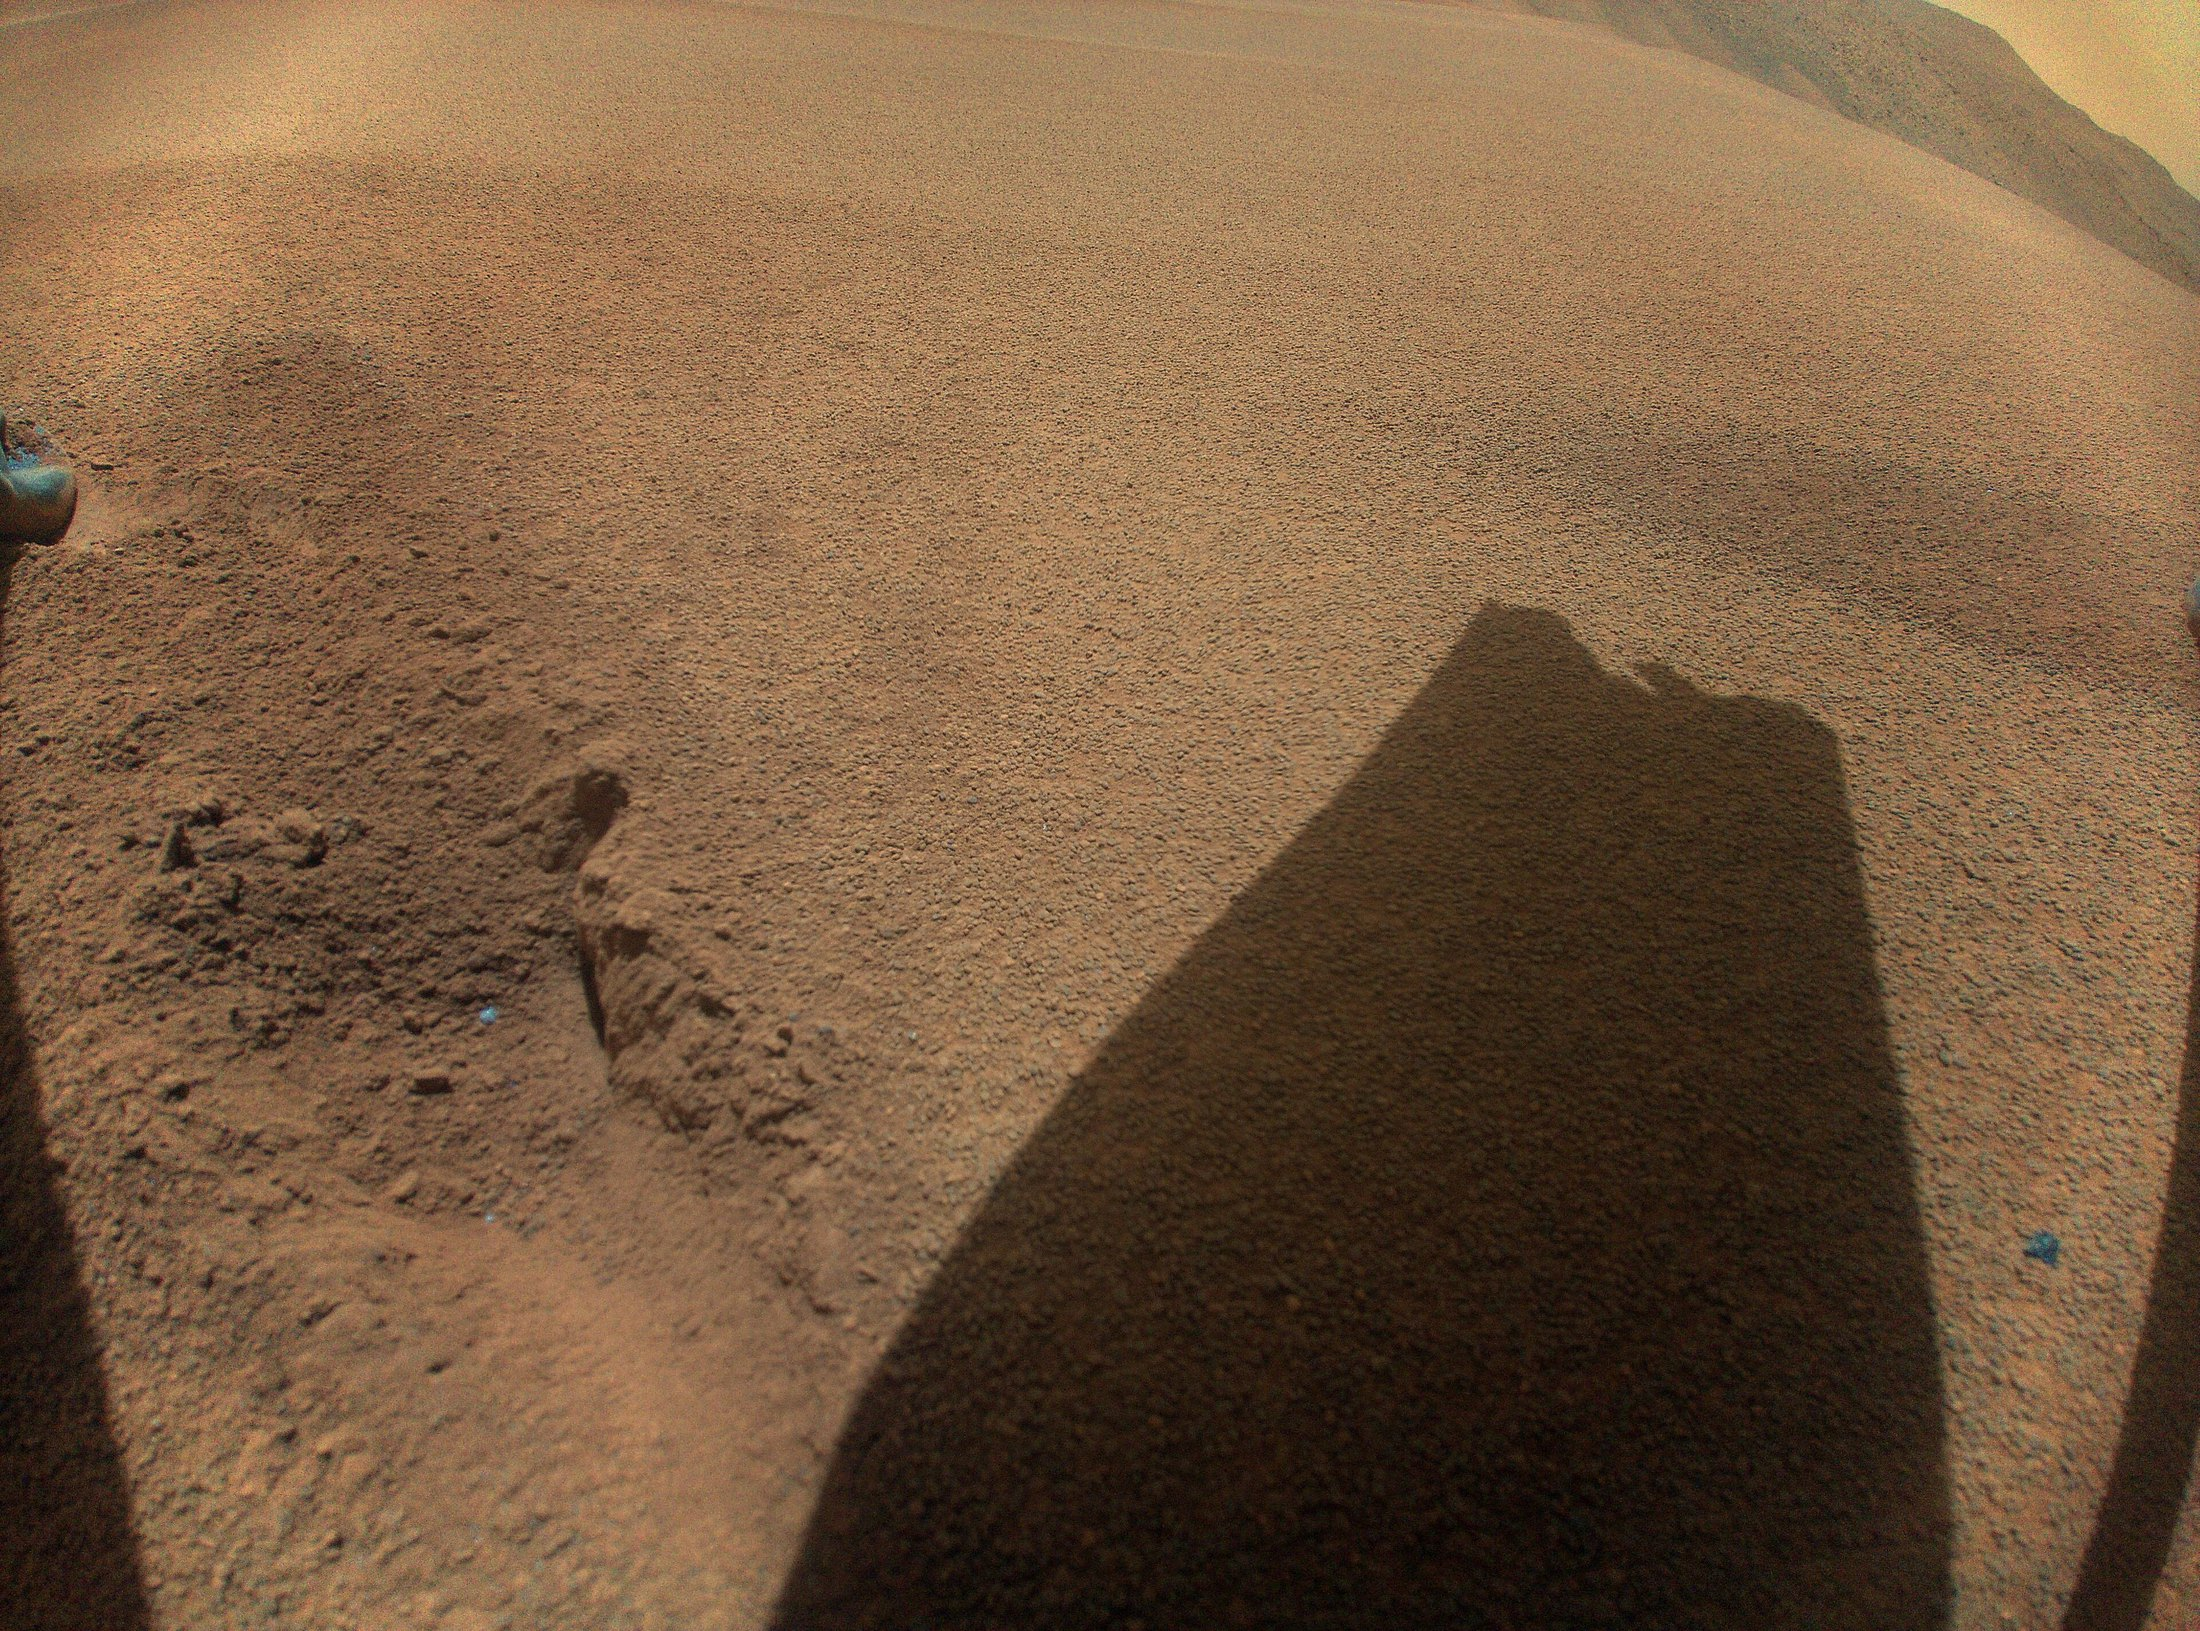
\includegraphics[height=40mm, trim=0 0 0 205, clip]{photos/ingenuity-blade}
  \captionsetup{style=sidecaption}
  \caption{Two pictures taken by Ingenuity's own camera, almost three years apart. Left: its shadow during the first flight, 19~April 2021. Right: the shadow of a broken rotor blade after the seventy-second and last, 18~January 2024. \hyperref[credit:ingenuity-shadow]{\textsc{credit}}, \hyperref[credit:ingenuity-blade]{\textsc{credit}}}
  \label{fig:intro-shadows}
\end{figure}

The flight I think of most is the sixth, on 22~May 2021. Fifty-four seconds after take-off a single image from the navigation camera was lost, and from then on every image arrived with the wrong time attached. The navigation kept \enquote{correcting} errors that did not exist. The helicopter began to tilt back and forth, with roll and pitch swings of more than twenty degrees, large commands to the rotors and spikes in power. It did not fall. It flew the rest of its route and landed about five metres from the planned spot. Its chief pilot, Håvard Grip, explained why a few days later:
\begin{quote}\itshape
We designed Ingenuity to tolerate significant errors without becoming unstable, including errors in timing. This built-in margin was not fully needed in Ingenuity's previous flights, because the vehicle's behavior was in-family with our expectations, but this margin came to the rescue in Flight Six.
\end{quote}
A margin — of stability, against errors nobody had foreseen — saved a machine hundreds of millions of kilometres from the nearest engineer. Much of this book is about what such a margin is and how to build one.

The seventy-second flight, on 18~January 2024, was the last. The helicopter crossed a stretch of smooth, featureless sand, where its navigation had little to track; on landing at least one rotor blade broke (Figure~\ref{fig:intro-shadows}, right). On 25~January NASA announced that the mission was over. Ingenuity still stands where it came down.

\section{From Mars to this book}

What kept Ingenuity in the air was not only its rotors, its batteries and its light carbon body. It was a loop: measure where you are, compare it with where you should be, act on the motors — and do it again, many times a second, faster than anything can go wrong. That loop is what this book is about, and almost every lesson in it is a piece of what Ingenuity had to do.

To hover, a rotorcraft must hold its height against gravity with a thrust it adjusts all the time; that is where the book starts (\lessonref{les:meet} to \lessonref{les:integral}). It must do it with motors that have limits, sensors that are noisy and a computer that looks at the world in snapshots (\lessonref{les:windup} to \lessonref{les:slow}). To move, or simply to stand still in a wind, it must tilt (\lessonref{les:tilt}), and so its loops are nested: a fast loop for its attitude inside a slower one for its position (\lessonref{les:cascade}). It must work out where it is from a camera and inertial sensors, none of which can be trusted alone (\lessonref{les:kalman}). And when something unforeseen happens — a lost image, a wrong timestamp — it must stay stable anyway, because its designers left a margin (\lessonref{les:edge}, and the whole of Part~III).

The drone of this book is a small cousin of Ingenuity. It has four rotors instead of two, and it flies not on Mars but in a simulator on your screen, where every experiment can be repeated, changed and broken without losing a spacecraft. The problems, though, are the same, and so are the ideas that solve them. My hope is that by the end of the book the reader will understand, in principle, how a machine like Ingenuity keeps itself in the air — and share a little of the admiration I felt watching it fly.\par
\smallskip
{\raggedleft\sffamily\small\color{muted}— Wojciech Stelmaszewski\par}

\section{What control is}

Look around you. The room you sit in is held at a comfortable temperature. Your body keeps its own temperature at \SI{37}{\celsius} whether you are in the sun or in the snow. The electricity in the socket arrives at 50 or \SI{60}{Hz}, never mind how many kettles were just switched on. A camera holds its picture still in a shaking hand. None of this happens by itself. Behind each of these facts is a \emph{control system}: something that measures, compares and acts, over and over again. This chapter is about the science of such systems.


Most of the physical world, left to itself, drifts. A room cools down, an engine speeds up when the load is removed, a pencil standing on its tip falls over. Engineering is very often the art of making such things behave the way we want them to, although we cannot know in advance everything that will happen to them.

\begin{definition}{Control}
\term{Control} is the act of choosing the inputs of a system so that its behaviour meets a goal, despite uncertainty about the system and about the influences acting on it. The system being controlled is called the \term{plant}; the device or algorithm that chooses the inputs is the \term{controller}.
\end{definition}

Every control problem has three ingredients:
\begin{enumerate}
  \item \textbf{a goal} — keep a temperature at \SI{21}{\celsius}, a car at \SI{100}{km/h}, a drone at \SI{2}{m};
  \item \textbf{a way to act} — a heater, a throttle, four motors (the \term{actuators});
  \item \textbf{uncertainty} — an open window, a hill, a gust of wind; and a model of the plant that is never quite right.
\end{enumerate}
Without the third ingredient there would be no subject. If we knew the plant exactly and nothing unexpected ever happened, we could compute the right inputs once, in advance, and simply play them back. Control theory exists because the world is uncertain.\didyouknow{The word \emph{plant} comes from the process industry: the first control engineers regulated chemical and power plants, and the name stayed — even when the plant is a drone, a patient or an economy.}

\subsection{Two ways to act: open loop and closed loop}
There are two fundamentally different ways to choose the inputs.

\begin{definition}{Open-loop and closed-loop control}
In \term{open-loop} control the input is computed from the goal and a model alone; the result is never checked. In \term{closed-loop} (\term{feedback}) control the result is measured by a \term{sensor}, compared with the goal, and the difference — the \term{error} — is used to correct the input continuously.
\end{definition}

A toaster is open-loop: it heats for a fixed time and never looks at the bread. Whether the toast comes out pale or burnt depends on the bread, the voltage and the starting temperature, and the toaster cannot tell. A thermostat is closed-loop: it measures the room temperature, compares it with the setting and switches the heater accordingly. Open the window, and the thermostat responds, without knowing that a window exists.\tip{To tell the two apart, ask one question: does the device look at the result? If it does not, it is open-loop, however clever its plan.}

\subsection{What feedback buys — and what it costs}
Feedback has four remarkable properties, and every one of them appears in this book.
\begin{enumerate}
  \item \textbf{It rejects disturbances it cannot see.} A controller reacts to the \emph{effect} of a disturbance, the error, so it does not need to know the cause (\lessonref{les:meet}).
  \item \textbf{It makes a system insensitive to its own imperfections.} This is less obvious and very important; the worked example below makes it concrete.
  \item \textbf{It can stabilise what is unstable.} A drone, a rocket balancing on its engine, a fighter jet designed to be unstable: none of them can stay up without feedback (\lessonref{les:edge}).
  \item \textbf{It can shape the behaviour} — speed, smoothness, damping — almost at will, by the choice of the controller.
\end{enumerate}
It also has costs. A feedback loop reacts only \emph{after} an error has appeared.\pitfall{The sign matters. Reverse the correction and the same loop pushes the error \emph{away} from zero. A microphone held close to its own loudspeaker howls for this reason.} It feeds the sensor's noise into the actuators (\lessonref{les:noise}). And, most importantly, a badly designed feedback loop can itself make a stable system oscillate or diverge: the Watt governors that \enquote{hunted}, and the bridge of \lessonref{les:spring}. Understanding exactly when feedback helps and when it harms is the core of control theory.

\begin{example}[Feedback makes an amplifier precise]
\label{ex:intro-black}
In 1927 the telephone engineer Harold Black\index{feedback amplifier}\index{Black, Harold} faced a problem: the vacuum-tube amplifiers of long-distance lines had a gain that drifted with temperature and age, and every drift distorted the calls. His solution was feedback, and a short calculation shows why it works.

\textbf{Step 1 — the open-loop amplifier.} Suppose an amplifier has a gain $A = 1000$, but, because of its tubes, the gain may vary by $\pm20\,\%$: anywhere between 800 and 1200. The output is $v_{out} = A\,v_{in}$, so the output varies by $\pm 20\,\%$ as well.

\textbf{Step 2 — close the loop.} Feed a fraction $\beta$ of the output back and subtract it from the input, using a precise resistor divider with $\beta = 0.1$.\didyouknow[-112pt]{Black had the idea on the ferry to work on 2~August 1927 and sketched it on his copy of \emph{The New York Times}. The patent took nine years to be granted: throwing gain away to gain precision sounded absurd.} The amplifier now amplifies the difference:
\begin{equation*}
  v_{out} = A\,(v_{in} - \beta\,v_{out}).
\end{equation*}

\textbf{Step 3 — solve for the closed-loop gain.} Collect $v_{out}$ on the left: $v_{out}(1 + A\beta) = A\,v_{in}$, so
\begin{equation*}
  G = \frac{v_{out}}{v_{in}} = \frac{A}{1 + A\beta}.
\end{equation*}

\textbf{Step 4 — put in the numbers.} For $A = 1000$: $G = 1000/101 = 9.901$. For $A = 800$: $G = 800/81 = 9.877$. For $A = 1200$: $G = 1200/121 = 9.917$.

\textbf{Step 5 — interpret.} The gain has dropped from 1000 to about 10, but its variation has dropped from $\pm20\,\%$ to about $\pm0.2\,\%$ — a hundred times smaller. When $A\beta \gg 1$, $G \approx 1/\beta$: the gain is set by the precise resistors, not by the imprecise tubes. We have traded raw gain for accuracy.\tip{A rule to keep: feedback divides every imperfection inside the loop by the loop gain. Here $1 + A\beta = 1 + 1000 \cdot 0.1 = 101$.} The factor $1 + A\beta$, by which the sensitivity drops, is called the \emph{loop gain}, and it will appear again and again, from \lessonref{les:droop} onwards.
\end{example}

\section{How control theory is organised}

Control theory is a large field, but its structure is simple. It follows the workflow of every control project (\cref{fig:intro-map}, top):
\begin{enumerate}
  \item \textbf{Modelling.} Write down equations that describe the plant well enough — Newton's laws for a drone, heat balances for a room, chemical kinetics for a reactor. Or measure the plant and fit a model to the data (\emph{system identification}).
  \item \textbf{Analysis.} Ask what the plant, and the plant with a given controller, will do: Is it stable? How fast does it respond? How much does a disturbance move it? How much can the model be wrong before things go bad?
  \item \textbf{Design.} Choose the controller so that the answers to these questions are acceptable. This is where the many families of methods differ.
  \item \textbf{Implementation.} Turn the design into something that runs: on a computer, at a finite sampling rate, with real sensors and actuators that are noisy, delayed and limited. Then test it — in simulation first — and go back to step 1 when reality disagrees.\didyouknow{Ask a practising control engineer where the time goes: mostly into modelling and testing. The control law itself is often a few dozen lines of code.}
\end{enumerate}

\begin{figure}[t]
\begin{fullwidth}
  \centering% A map of control theory: the workflow (top) and the families of methods (below), with the course's lessons.
\begin{tikzpicture}[
  every node/.style={font=\sffamily\footnotesize},
  wfstep/.style={draw=ink, line width=0.6pt, rounded corners=2pt, fill=white, minimum height=12.5mm, text width=33.2mm, align=center, inner sep=3pt},
  fam/.style={draw=#1, line width=0.6pt, rounded corners=2pt, fill=#1!7, text width=48.9mm, align=left, inner sep=5pt,
    minimum height=25mm, anchor=north west},
]
  % workflow: four equal steps across the full width
  \node[wfstep, anchor=north west] (m) at (0,0) {\textbf{Model}\\{\scriptsize\color{muted}equations of the plant}};
  \node[wfstep, anchor=north west] (a) at (43.5mm,0) {\textbf{Analyse}\\{\scriptsize\color{muted}stability, speed, margins}};
  \node[wfstep, anchor=north west] (d) at (87mm,0) {\textbf{Design}\\{\scriptsize\color{muted}the control law}};
  \node[wfstep, anchor=north west] (i) at (130.5mm,0) {\textbf{Implement and test}\\{\scriptsize\color{muted}sample, filter, saturate}};
  \draw[sig] (m) -- (a); \draw[sig] (a) -- (d); \draw[sig] (d) -- (i);
  \draw[sig, faint] (i.north) -- ++(0,4mm) -| node[pos=0.25, above, lab] {not good enough? iterate} (m.north);
  % families: two rows of three, tops and heights aligned
  \node[font=\sffamily\scriptsize, text=muted, anchor=south west, inner sep=0pt] at (0,-21mm) {families of methods — each answers the design question differently};
  \node[fam=sigP]     at (0,-23mm)       {\textcolor{sigP}{\textbf{Classical}}\\ PID, frequency response, Bode and Nyquist, root locus\\[2pt]{\color{muted}Lessons 1–14}\\{\color{faint}later: III.1–III.6}};
  \node[fam=deepblue] at (56.67mm,-23mm)    {\textcolor{deepblue}{\textbf{State space}}\\ state feedback, observers, LQR, Kalman filter\\[2pt]{\color{muted}Lessons II.1–II.4}\\{\color{faint}later: III.9–III.10}};
  \node[fam=sigI]     at (113.33mm,-23mm)   {\textcolor{sigI}{\textbf{Nonlinear and geometric}}\\ Lyapunov, dynamic inversion, rotations, flatness\\[2pt]{\color{muted}Lessons II.7–II.12}\\{\color{faint}later: III.7–III.8}};
  \node[fam=sigD]     at (0,-52mm)       {\textcolor{sigD}{\textbf{Optimal and predictive}}\\ Pontryagin, dynamic programming, MPC\\[2pt]{\color{muted}Lessons II.2, II.13–II.17}\\{\color{faint}later: IV.1–IV.6}};
  \node[fam=sigFF]    at (56.67mm,-52mm)    {\textcolor{sigFF}{\textbf{Robust and adaptive}}\\ disturbance observers, ADRC, L1 adaptive, $H_\infty$\\[2pt]{\color{muted}Lessons II.5–II.6, II.18}\\{\color{faint}later: III.11–III.17}};
  \node[fam=sigerr]   at (113.33mm,-52mm)   {\textcolor{sigerr}{\textbf{Learning-based}}\\ learned models, reinforcement learning, neural policies\\[2pt]{\color{muted}Lessons II.19–II.21}\\{\color{faint}later: III.29–III.30}};
\end{tikzpicture}

  \caption{A map of control theory. Top: the workflow that every control design follows. Below: the main families of design methods, roughly in the order they were developed, with the lessons of this book in which they appear. The fainter line names the lessons of Parts~III and~IV, in later volumes, that return to each family.}
  \label{fig:intro-map}
\end{fullwidth}
\end{figure}

The families of design methods in \cref{fig:intro-map} are not rival schools; they are layers, each added when the previous ones reached their limits.
\begin{description}[leftmargin=0pt, itemsep=3pt, font=\sffamily\small\bfseries]
  \item[Classical control] (1920s–1950s) works with one input and one output and describes systems by how they respond to sinusoids of different frequencies. Its workhorse, the PID controller, still runs the vast majority of the world's control loops.\innumbers{Surveys of process plants find that more than nine loops in ten are PID — and most of those are really PI, with the D term switched off.} Part~I of this book.
  \item[State-space control] (from 1960) describes a system by a vector of internal variables, its \emph{state}, and handles many inputs and outputs at once with linear algebra. It brought optimal control (LQR) and optimal estimation (the Kalman filter).
  \item[Nonlinear and geometric control] deals with systems whose equations cannot be linearised usefully — large rotations, for example, which matter for every aircraft and drone.
  \item[Optimal and predictive control] states the goal as a cost to be minimised and computes the control by optimisation, often online, while respecting limits such as maximum thrust or forbidden regions.
  \item[Robust and adaptive control] designs controllers that keep working when the model is wrong: either by being insensitive to the error (robust) or by learning it during operation (adaptive).
  \item[Learning-based control] uses data and machine learning to build models, or to learn the controller itself.
\end{description}
Part~II of this book walks through all of them, on the same drone. It teaches each family as a way to \emph{design} a controller. The analysis that says in advance whether a design will work — the frequency response, Lyapunov's method, robustness to a wrong model — is the subject of Part~III, and the optimal-control theory of Pontryagin and Bellman, together with vehicles that a drone cannot imitate, of Part~IV. Those parts follow in later volumes.

\section{Where control matters}

It is hard to name a branch of engineering that does not depend on feedback. A few examples, with what is measured and what is acted upon, show the range:

\begin{center}\small
\renewcommand{\arraystretch}{1.25}
\begin{tabularx}{\linewidth}{@{}>{\sffamily\bfseries}p{23mm}>{\raggedright\arraybackslash}X>{\raggedright\arraybackslash}p{36mm}@{}}
\toprule
\normalfont\sffamily field & example & measure $\rightarrow$ act on\\
\midrule
aerospace & autopilots, fly-by-wire, rocket landing, satellite pointing & attitude, position $\rightarrow$ control surfaces, engines\\
automotive & cruise control, anti-lock brakes, stability control, engine management & wheel speed, oxygen in the exhaust $\rightarrow$ brakes, fuel injection\\
energy & grid frequency, wind-turbine pitch, power electronics & frequency, rotor speed $\rightarrow$ valves, blade angle, switches\\
process industry & refineries, chemical reactors, paper mills & temperature, pressure, flow $\rightarrow$ valves, pumps\\
robotics \& machines & industrial arms, CNC machines, hard-disk heads, 3D printers & joint angles, head position $\rightarrow$ motor currents\\
medicine & insulin pumps (artificial pancreas), anaesthesia, pacemakers & blood glucose, heart rhythm $\rightarrow$ insulin, pacing pulses\\
computing & network congestion control, server autoscaling & packet loss, load $\rightarrow$ sending rate, number of servers\\
economics & inflation targeting by central banks & inflation $\rightarrow$ interest rate\\
biology & body temperature, blood pressure, posture — \emph{homeostasis} & nerve signals $\rightarrow$ muscles, hormones\\
\bottomrule
\end{tabularx}
\end{center}

The last row is a reminder that engineers did not invent feedback; they rediscovered it. Living organisms are full of control loops, and the physiologist Walter Cannon's word for them, \emph{homeostasis} (1926), means almost exactly what \emph{Anemostatos} means: standing still — in the wind of the outside world.\innumbers{Your own loop: your body temperature stays within about half a degree while the air around you may vary by fifty.}

\section{A short history}

\begin{figure}[p]
\begin{fullwidth}
  \centering% History timeline (generated by hand-written list in the book sources)
\begin{tikzpicture}[yscale=1.13, every node/.style={font=\sffamily\footnotesize}]
\def\rowh{9.2mm}
\fill[sigFF] (0,0.0mm) circle (1.5pt);
\node[anchor=east, text=sigFF, font=\sffamily\footnotesize\bfseries] at (-3mm,0.0mm) {c. 270 BC};
\node[anchor=west, text width=113mm, align=left] at (4mm,0.0mm) {Ktesibios of Alexandria regulates the water level of a clock with a float valve — the oldest known feedback device.};
\node[anchor=east, text=sigFF, font=\sffamily\scriptsize\scshape] at (-24mm,0.0mm) {mechanical};
\fill[sigFF] (0,-9.2mm) circle (1.5pt);
\node[anchor=east, text=sigFF, font=\sffamily\footnotesize\bfseries] at (-3mm,-9.2mm) {1620s};
\node[anchor=west, text width=113mm, align=left] at (4mm,-9.2mm) {Cornelis Drebbel keeps an egg incubator at constant temperature with a mercury thermostat.};
\fill[sigFF] (0,-18.4mm) circle (1.5pt);
\node[anchor=east, text=sigFF, font=\sffamily\footnotesize\bfseries] at (-3mm,-18.4mm) {1788};
\node[anchor=west, text width=113mm, align=left] at (4mm,-18.4mm) {James Watt fits the centrifugal governor to his steam engines.};
\fill[deepblue] (0,-27.599999999999998mm) circle (1.5pt);
\node[anchor=east, text=deepblue, font=\sffamily\footnotesize\bfseries] at (-3mm,-27.599999999999998mm) {1868};
\node[anchor=west, text width=113mm, align=left] at (4mm,-27.599999999999998mm) {James Clerk Maxwell, \emph{On Governors}: the first mathematical analysis of a feedback loop.};
\node[anchor=east, text=deepblue, font=\sffamily\scriptsize\scshape] at (-24mm,-27.599999999999998mm) {mathematical};
\fill[deepblue] (0,-36.8mm) circle (1.5pt);
\node[anchor=east, text=deepblue, font=\sffamily\footnotesize\bfseries] at (-3mm,-36.8mm) {1877–1895};
\node[anchor=west, text width=113mm, align=left] at (4mm,-36.8mm) {Edward Routh and Adolf Hurwitz: stability from the coefficients of a polynomial.};
\fill[deepblue] (0,-46.0mm) circle (1.5pt);
\node[anchor=east, text=deepblue, font=\sffamily\footnotesize\bfseries] at (-3mm,-46.0mm) {1892};
\node[anchor=west, text width=113mm, align=left] at (4mm,-46.0mm) {Aleksandr Lyapunov: stability of nonlinear motion, without solving the equations.};
\fill[sigP] (0,-55.199999999999996mm) circle (1.5pt);
\node[anchor=east, text=sigP, font=\sffamily\footnotesize\bfseries] at (-3mm,-55.199999999999996mm) {1922};
\node[anchor=west, text width=113mm, align=left] at (4mm,-55.199999999999996mm) {Nicolas Minorsky describes the three-term (PID) controller for ship steering.};
\node[anchor=east, text=sigP, font=\sffamily\scriptsize\scshape] at (-24mm,-55.199999999999996mm) {electronic};
\fill[sigP] (0,-64.39999999999999mm) circle (1.5pt);
\node[anchor=east, text=sigP, font=\sffamily\footnotesize\bfseries] at (-3mm,-64.39999999999999mm) {1927};
\node[anchor=west, text width=113mm, align=left] at (4mm,-64.39999999999999mm) {Harold Black invents the negative-feedback amplifier at Bell Labs.};
\fill[sigP] (0,-73.6mm) circle (1.5pt);
\node[anchor=east, text=sigP, font=\sffamily\footnotesize\bfseries] at (-3mm,-73.6mm) {1932–1945};
\node[anchor=west, text width=113mm, align=left] at (4mm,-73.6mm) {Harry Nyquist's stability criterion; Hendrik Bode's frequency-response design.};
\fill[sigP] (0,-82.8mm) circle (1.5pt);
\node[anchor=east, text=sigP, font=\sffamily\footnotesize\bfseries] at (-3mm,-82.8mm) {1942};
\node[anchor=west, text width=113mm, align=left] at (4mm,-82.8mm) {Ziegler and Nichols publish their tuning rules; PID spreads through industry.};
\fill[sigP] (0,-92.0mm) circle (1.5pt);
\node[anchor=east, text=sigP, font=\sffamily\footnotesize\bfseries] at (-3mm,-92.0mm) {1948};
\node[anchor=west, text width=113mm, align=left] at (4mm,-92.0mm) {Norbert Wiener, \emph{Cybernetics}; Walter Evans, the root locus.};
\fill[sigmeas] (0,-101.19999999999999mm) circle (1.5pt);
\node[anchor=east, text=sigmeas, font=\sffamily\footnotesize\bfseries] at (-3mm,-101.19999999999999mm) {1956–1960};
\node[anchor=west, text width=113mm, align=left] at (4mm,-101.19999999999999mm) {Pontryagin's maximum principle, Bellman's dynamic programming, Kalman's state space, LQR and filter.};
\node[anchor=east, text=sigmeas, font=\sffamily\scriptsize\scshape] at (-24mm,-101.19999999999999mm) {space age};
\fill[sigmeas] (0,-110.39999999999999mm) circle (1.5pt);
\node[anchor=east, text=sigmeas, font=\sffamily\footnotesize\bfseries] at (-3mm,-110.39999999999999mm) {1961–1972};
\node[anchor=west, text width=113mm, align=left] at (4mm,-110.39999999999999mm) {Apollo: digital guidance, Kalman filtering in flight, the first digital autopilots.};
\fill[sigI] (0,-119.6mm) circle (1.5pt);
\node[anchor=east, text=sigI, font=\sffamily\footnotesize\bfseries] at (-3mm,-119.6mm) {1970s–80s};
\node[anchor=west, text width=113mm, align=left] at (4mm,-119.6mm) {Model predictive control in oil refineries; robust control ($H_\infty$); digital fly-by-wire in airliners (A320, 1988).};
\node[anchor=east, text=sigI, font=\sffamily\scriptsize\scshape] at (-24mm,-119.6mm) {computers};
\fill[sigI] (0,-128.79999999999998mm) circle (1.5pt);
\node[anchor=east, text=sigI, font=\sffamily\footnotesize\bfseries] at (-3mm,-128.79999999999998mm) {2000s};
\node[anchor=west, text width=113mm, align=left] at (4mm,-128.79999999999998mm) {Cheap MEMS sensors and microcontrollers: the quadrotor becomes a toy, a camera and a research platform.};
\fill[sigD] (0,-138.0mm) circle (1.5pt);
\node[anchor=east, text=sigD, font=\sffamily\footnotesize\bfseries] at (-3mm,-138.0mm) {2010s–today};
\node[anchor=west, text width=113mm, align=left] at (4mm,-138.0mm) {Optimisation and learning in the loop: rockets landing themselves, reinforcement-learned policies that beat human drone racers (2023).};
\node[anchor=east, text=sigD, font=\sffamily\scriptsize\scshape] at (-24mm,-138.0mm) {learning};
\draw[sigFF, line width=1.2pt] (0,0.0mm) -- (0,-9.2mm);
\draw[sigFF, line width=1.2pt] (0,-9.2mm) -- (0,-18.4mm);
\draw[sigFF, line width=1.2pt] (0,-18.4mm) -- (0,-27.599999999999998mm);
\draw[deepblue, line width=1.2pt] (0,-27.599999999999998mm) -- (0,-36.8mm);
\draw[deepblue, line width=1.2pt] (0,-36.8mm) -- (0,-46.0mm);
\draw[deepblue, line width=1.2pt] (0,-46.0mm) -- (0,-55.199999999999996mm);
\draw[sigP, line width=1.2pt] (0,-55.199999999999996mm) -- (0,-64.39999999999999mm);
\draw[sigP, line width=1.2pt] (0,-64.39999999999999mm) -- (0,-73.6mm);
\draw[sigP, line width=1.2pt] (0,-73.6mm) -- (0,-82.8mm);
\draw[sigP, line width=1.2pt] (0,-82.8mm) -- (0,-92.0mm);
\draw[sigP, line width=1.2pt] (0,-92.0mm) -- (0,-101.19999999999999mm);
\draw[sigmeas, line width=1.2pt] (0,-101.19999999999999mm) -- (0,-110.39999999999999mm);
\draw[sigmeas, line width=1.2pt] (0,-110.39999999999999mm) -- (0,-119.6mm);
\draw[sigI, line width=1.2pt] (0,-119.6mm) -- (0,-128.79999999999998mm);
\draw[sigI, line width=1.2pt] (0,-128.79999999999998mm) -- (0,-138.0mm);
\end{tikzpicture}

  \par\vspace{9mm}
  % six portraits cropped to one frame, 25 mm by 31 mm
  \newcommand{\portrait}[2]{\begin{minipage}[t]{25mm}\raggedright
    \includegraphics[width=25mm]{photos/portrait-#1}\par\vspace{3pt}
    {\sffamily\scriptsize\color{muted}#2\\\hyperref[credit:#1]{\textsc{credit}}\par}\end{minipage}}
  \noindent
  \portrait{ctesibius}{Ktesibios's water clock, as drawn in 1854}\hfill
  \portrait{maxwell}{James Clerk Maxwell, 1831–1879}\hfill
  \portrait{bode}{Hendrik Bode, 1905–1982}\hfill
  \portrait{wiener}{Norbert Wiener, 1894–1964}\hfill
  \portrait{pontryagin}{Lev Pontryagin, 1908–1988}\hfill
  \portrait{kalman}{Rudolf Kálmán, 1930–2016}
  \par\vspace{4pt}
  \caption{Twenty-three centuries of feedback. The colours mark the eras described in the text; below, six of the people and devices named there.}
  \label{fig:intro-timeline}
\end{fullwidth}
\end{figure}
The history of control (\cref{fig:intro-timeline}) is a story of practice running ahead of theory, and theory catching up in bursts.

\paragraph{The mechanical era.} Feedback devices are ancient. Around 270~BC Ktesibios of Alexandria\index{Ktesibios of Alexandria} kept the water level in a clock constant with a float that closed the inflow when the level rose — the ancestor of the float valve in every toilet cistern. In the 1620s Cornelis Drebbel\index{Drebbel, Cornelis} built an incubator whose temperature regulated itself. The industrial revolution produced the most famous device of all, Watt's centrifugal governor of 1788\index{centrifugal governor}\index{Watt, James} (\lessonref{les:meet}), and thousands of steam engines carried it.

\paragraph{The mathematical era.} Governors sometimes \emph{hunted}, oscillating instead of settling, and nobody knew why. In 1868 James Clerk Maxwell\index{Maxwell, James Clerk} wrote down the linearised equations of a governor and showed that stability depends on the roots of a polynomial;\didyouknow{Maxwell could decide stability only up to the third order. The general question was set for the Adams Prize at Cambridge; Routh won it in 1877.} Edward Routh (1877)\index{Routh, Edward} and Adolf Hurwitz (1895)\index{Hurwitz, Adolf} found how to decide it from the coefficients alone, and Aleksandr Lyapunov (1892)\index{Lyapunov, Aleksandr} extended the idea to nonlinear systems. These results are the backbone of \lessonref{les:spring} and \lessonref{les:damper}.

\paragraph{The electronic era.} In the 1920s and 1930s telephony and ships brought new problems. Nicolas Minorsky described\index{Minorsky, Nicolas} the PID controller\index{PID controller!history} for steering ships (1922, \lessonref{les:integral}); Harold Black invented the feedback amplifier (1927, Example~\ref{ex:intro-black}); at Bell Laboratories Harry Nyquist (1932)\index{Nyquist, Harry} and Hendrik Bode (1940s)\index{Bode, Hendrik} created the frequency-domain methods that let engineers design loops with pencil and paper. The Second World War — radar-guided guns, autopilots — turned these ideas into a discipline, and in 1948 Norbert Wiener\index{Wiener, Norbert} gave it a name, \emph{cybernetics}, and a place among the sciences.

\paragraph{The space age.} Around 1960 three results appeared almost at once: Lev Pontryagin's maximum principle\index{Pontryagin, Lev}\index{Pontryagin's maximum principle} and Richard Bellman's dynamic programming\index{Bellman, Richard}\index{dynamic programming} for optimal control, and Rudolf Kálmán's state-space theory\index{Kálmán, Rudolf}, with the linear-quadratic regulator and the Kalman filter. They arrived just in time for the space race. The Apollo spacecraft navigated to the Moon with a Kalman filter\index{Apollo guidance computer} running on its on-board computer,\innumbers{The Apollo guidance computer: \SI{32}{kg}, about 2\,000 words of erasable memory and 36\,000 words of program woven by hand into magnetic cores.} and a spare Apollo computer then flew the first digital fly-by-wire aircraft (\lessonref{les:slow}).

\paragraph{The computer era.} As computers became cheap, control moved into software. From the late 1970s oil refineries began to run \emph{model predictive control}, solving an optimisation problem every few minutes to plan their valves; robust control theory addressed models that are known only approximately; digital fly-by-wire entered airliners with the Airbus A320 in 1988. Cheap micro-electro-mechanical sensors and microcontrollers made the multicopter possible in the 2000s.

\paragraph{Today.} Optimisation and learning now run inside fast loops. Rockets land on floating platforms by solving an optimisation problem in real time, and in 2023 a quadrotor flown by a neural network trained with reinforcement learning beat human world champions in drone racing.\innumbers{The racing policy learned from about three weeks of flying — simulated in under an hour on one workstation.} And still, underneath almost all of it, there are PID loops, running exactly as Minorsky described them a hundred years ago.

\section{Why learn it — and why on a drone}

Control theory is worth learning for a practical reason and for a deeper one. The practical reason is the table above: whatever you build that moves, heats, flows or computes, it will sooner or later need a feedback loop, and a loop designed without understanding is a loop that oscillates in the field. The deeper reason is that control theory is a way of thinking about dynamic systems that transfers between fields: the same equations describe a drone, a reactor and a central bank, and the same questions — is it stable? how fast? how robust? — apply to all of them.

\subsection{The drone as a laboratory}
Why learn it on a quadrotor rather than on a heater or a tank? Because a hovering drone is a nearly perfect teaching plant.
\begin{itemize}
  \item \textbf{It is unstable without control.} Switch the controller off and it falls within a second. Every mistake is visible immediately, and there is no way to hide behind a plant that would have been fine on its own.
  \item \textbf{Its physics is simple and familiar.} Newton's second law — force equals mass times acceleration — is enough for Part~I. You do not need to learn chemistry or thermodynamics first.
  \item \textbf{It is fast.} Its dynamics play out in seconds, so experiments take seconds too. A room heater would need hours.\innumbers{Falling from rest, a drone drops \SI{4.9}{m} in its first second. A human needs a fifth of a second to react: \SI{20}{cm} are gone before a finger moves.}
  \item \textbf{It grows with you.} Restricted to vertical motion it is the simplest non-trivial plant there is: a mass pushed by a force. Released into three dimensions it becomes a rigid body with rotations, a chain of four integrators, and coupled, nonlinear dynamics — enough to motivate every family of methods in \cref{fig:intro-map}.
  \item \textbf{It meets every real-world problem.} Its motors saturate and lag, its sensors are noisy, its controller samples, the wind is random, its payload changes, its propellers break. Each of these problems has its own lesson.
\end{itemize}

\begin{example}[How much can go wrong in one second]
Here is a first taste of why a drone needs feedback, with numbers you will meet again in \lessonref{les:meet}.

\textbf{Step 1 — the plan.} A \SI{1}{kg} drone should hover. Newton's law along the vertical, with thrust $T$ and gravity $mg$, is $m\ddot y = T - mg$. Hovering means $\ddot y = 0$, so the plan is $T = mg = 1 \cdot 9.81 = \SI{9.81}{N}$.

\textbf{Step 2 — a small error.} The battery is \SI{2}{\%} heavier than we assumed: $m = \SI{1.02}{kg}$. The weight is now $1.02 \cdot 9.81 = \SI{10.006}{N}$, but we still apply \SI{9.81}{N}. The net force is $9.81 - 10.006 = \SI{-0.196}{N}$.

\textbf{Step 3 — the acceleration.} $\ddot y = -0.196/1.02 = \SI{-0.192}{m/s^2}$: small, and constant.

\textbf{Step 4 — integrate twice.} Starting at rest, $\dot y(t) = -0.192\,t$ and $y(t) = y_0 - \tfrac12\,0.192\,t^2$.

\textbf{Step 5 — evaluate.} After \SI{1}{s} the drone has sunk \SI{9.6}{cm}; after \SI{5}{s}, \SI{2.4}{m} — it has hit the floor from a hover at two metres. A two-percent error in one number has become a crash in five seconds.\pitfall[-14pt]{Open-loop errors do not stay small. A constant error in force becomes an error in position that grows as $t^2$.} No model is ever that good, and the wind has not even started blowing. Feedback is not optional.
\end{example}

\subsection{What you will be able to do}
By the end of Part~I you will be able to explain every term of a PID controller physically, predict its behaviour with a few lines of algebra, diagnose the classic practical problems from a plot, and tune a cascade of loops for a vehicle that moves in three dimensions. By the end of Part~II you will know what the modern alternatives to PID do, what each of them costs, and how to choose between them. The later parts of the course add what an engineer needs before a design may fly: by the end of Part~III, to say how far a loop is from instability and how wrong its model may be; by the end of Parts~IV and~V, to do the same for an aircraft, a rocket and a satellite, and to verify the result.

\subsection{How to study with this book}
Each lesson is designed to be read with the simulator open. A good rhythm is:
\begin{enumerate}
  \item read the lesson up to the first \emph{Try this} box;
  \item before touching the simulator, answer the \emph{Predict first} question on paper;\tip{Write the prediction down. A guess you did not commit to cannot surprise you.}
  \item run the experiment, and compare what you see with what you predicted — the surprises are where the learning happens;
  \item work through the worked examples with a pencil, then try the exercises on your own.
\end{enumerate}
The mathematics is always developed step by step, from what a bachelor's degree provides. When a step uses a tool you have not seen, it is explained where it is used and collected in the \hyperref[app:math]{mathematical toolbox} at the end of the book.
